% Copyright (C) 2019 Cui Jialiang ( SESS, PKU ). All rights reserved.

\chapter{结果,结论与讨论}
本章将主要介绍本文为验证本文的实验(见\ref{section:experiment})的结果,本研究的结论,与本研究引发的讨论.
\section{实验结果与结论}
本研究的实验顺利进行了,并得到了结果.
\subsection{实验结果图像展示}
\par
\begin{sidewaysfigure}[htbp!]
    \centering
    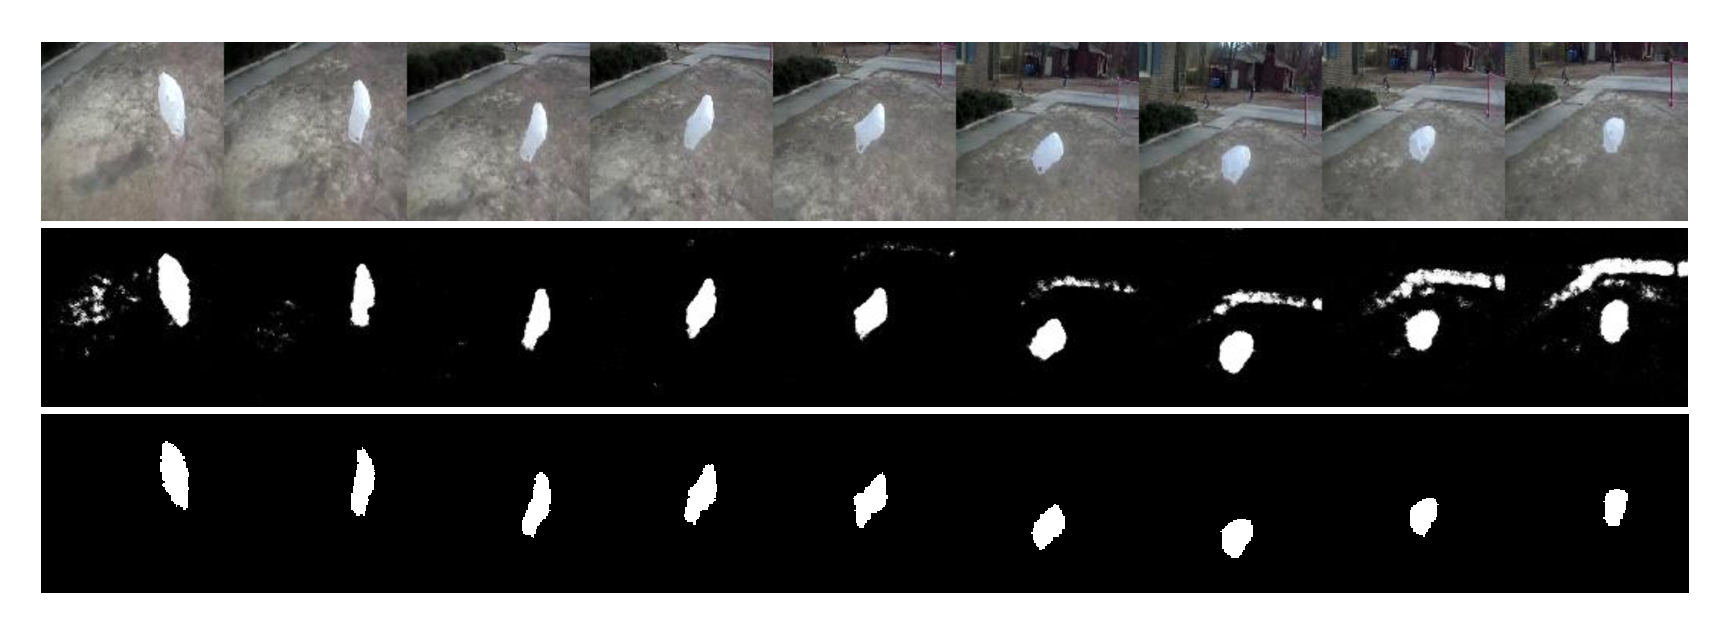
\includegraphics[width = 1.\textwidth]{chap/img/result_bag.pdf}
    \caption{跟踪结果-袋子:第一行为原图,第二行为跟踪结果概率图,第三行为二值化结果}
    \label{fig:result_bag}
\end{sidewaysfigure}
\par
\begin{sidewaysfigure}[htbp!]
    \centering
    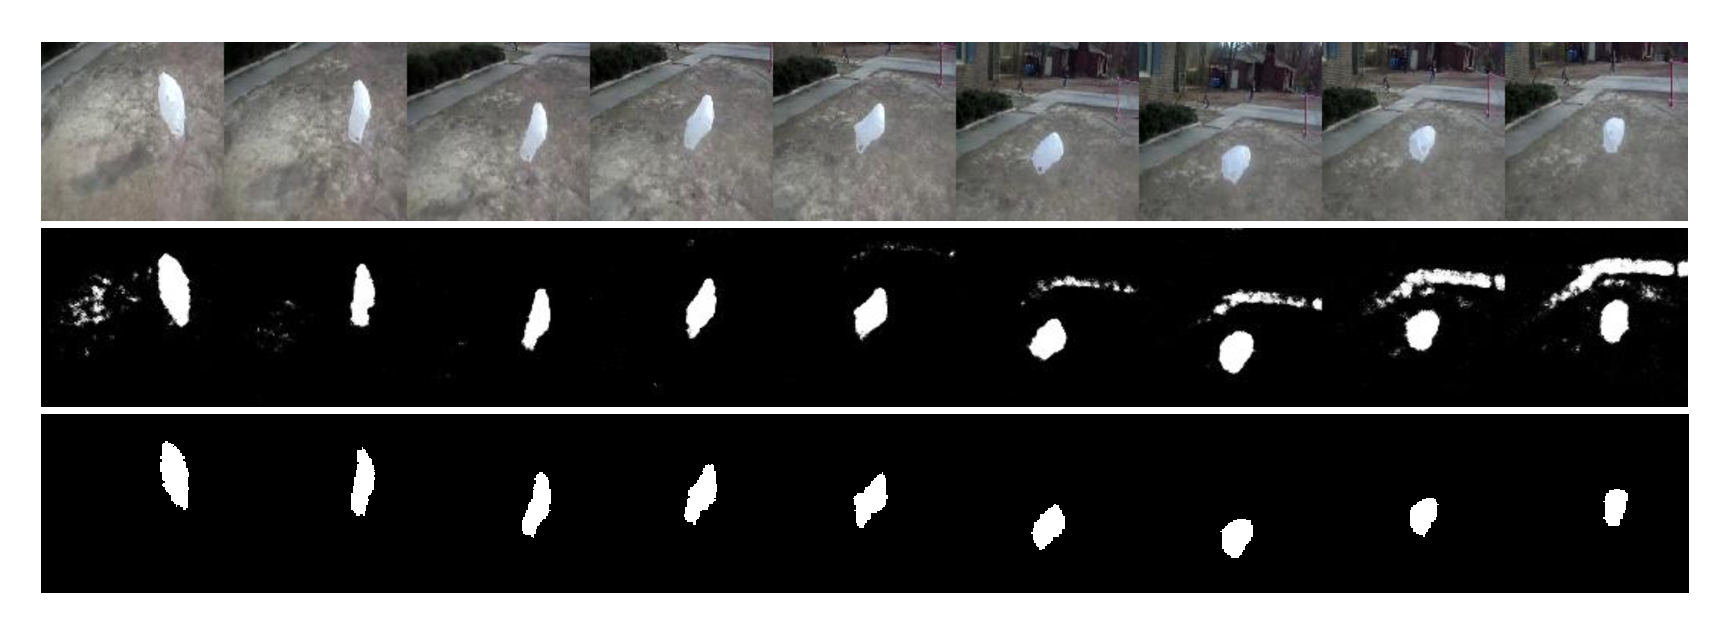
\includegraphics[width = 1.\textwidth]{chap/img/result_bag.pdf}
    \caption{跟踪结果-老虎玩具:第一行为原图,第二行为跟踪结果概率图,第三行为二值化结果}
    \label{fig:result_tiger}
\end{sidewaysfigure}
\par
实验结果的图像展示见图\ref{fig:result_bag}和图\ref{fig:result_tiger}.
\par
\subsection{实验结果定量评估}
\par
\begin{sidewaysfigure}[htbp!]
    \centering
    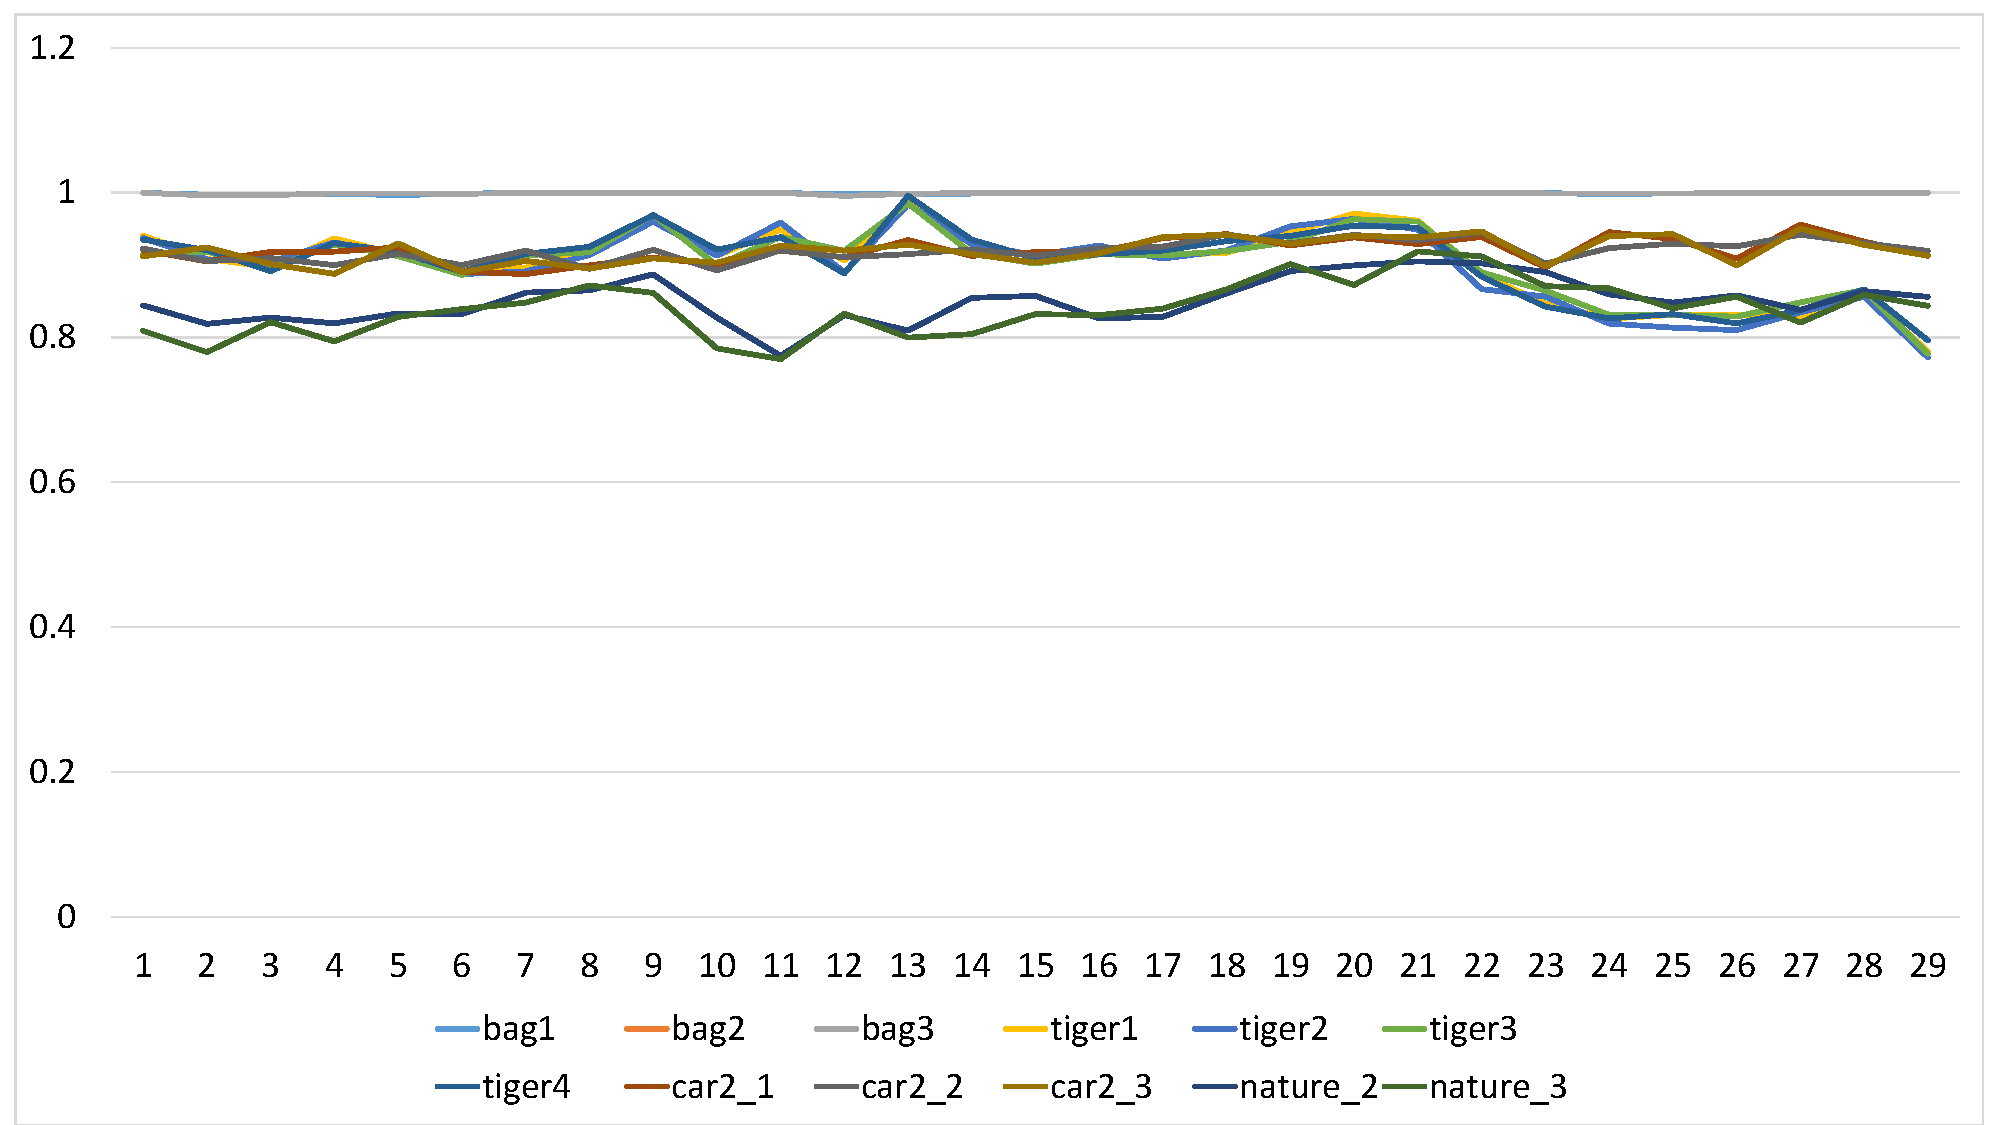
\includegraphics[width = 1.\textwidth]{chap/img/res_auc.pdf}
    \caption{测试集中一些序列的跟踪AUC统计}
    \label{fig:res_auc}
\end{sidewaysfigure}
\par
本实验采用了AUC作为评价结果(详见前文\ref{section:auc}).图\ref{fig:res_auc}中展示了几组实验的AUC统计.
\par
可以看到,在许多样本序列中,本研究的模型具有一定的跟踪能力.
\subsection{实验结论}
经过实验,本研究提出的像素级目标跟踪算法具有一定的像素级目标跟踪能力,具有应用的前景与希望.

\section{总结与讨论}
本节将总结研究的结论,分析并罗列本研究的创新点与不足,并对接下来的工作进行展望.
\par
本研究提出了一种基于CNN和RNN的像素级目标跟踪算法,主要运用了深度学习技术中的循环神经网络与加-解码结构;实现并用数据进行了实验,得到了较好的实验结果.
\subsection{本研究的创新点}
本研究第一次在有物理依据的情况下将RNN插入加密-解码结构的各个层级.这种结构对于处理多尺度图像处理问题将有创新效应.过去的研究中CNN与RNN的结合方式大多是先用CNN得到向量结果,再用RNN对这个结果进行处理.本文的思路会为RNN保留更多的空间信息.
\par
近年来像素级别的跟踪一直缺乏研究,而像素级的跟踪更加贴近跟踪本质.本研究的进行有利于推动像素级跟踪算法的研究与迭代.
\subsection{本研究的不足}
由于数据集的限制,本研究实验时采用的训练与测试数据序列都太短,还未达到实际应用需要的长度.这需要更长视频的数据集的支持.
\par
本研究进行的实验较有限,一方面受数据集的范围限制,另一方面受硬件限制,无法进行更大规模的训练.本研究将图像采样至$500*500$大小,实际上是由于平台内存不足的无奈之举.如果输入图像可以更大,像素级跟踪得到的结果就会更精致,处理过程中的信息损失也会更小.
\par
也由于平台与实验时间限制,本研究的实验只实现了3层的加密-解码结构.目前通常图像分割会采用5层以上的加密-解码结构,以保证深层的CNN能获取更加全局的信息.本文虽然使用Conv-LSTM结构处理了全局信息,但如果能在加密-解码结构中增加更多的全局信息,将对解码过程有巨大的帮助.
\subsection{后续工作}
本文的后续工作将在以下几个方面进行:
\begin{itemize}
    \item 添加更多数据,得到更多实验结果.
    \item 尝试更深层次的加密-解码结构,与更大的初始图像处理.
    \item 尝试真实应用场景的数据的跟踪效果.
    \item 尝试调整模型参数以求得到更好的效果.
    \item 尝试微调模型结构,如加密-解码结构与RNN的结合层数等.
    \item 尝试该结构(RNN加入各级加密-解码结构)在其它问题,如视频目标分割,视频稳定\supercite{benchme}等场景的应用.
\end{itemize}

\subsection{展望}
本文证明了加入了RNN结构的加密-解码模型在像素级目标跟踪问题上的效果,也发掘了像素级别目标跟踪问题的研究空间.根据目前的研究趋势,像素级以及矩形级的目标跟踪的推动都主要依靠深度学习算法.
\par
近期的深度学习研究主要在修改深度神经网络的模型结构,以求得到更适应问题的神经网络,并得到更好的结果.神经网络结构的改进包括基础网络单元,如CNN,RNN,以及本文的块状CNN,也包括各种基础网络单元结构的组合方式.
\par
对于跟踪问题,本研究中认为迫切需要解决的网络结构问题有:
\begin{itemize}
    \item 更好的RNN单元,更能保留有效信息,更好的长效处理.
    \item 更有效的RNN与CNN结合方式.
    \item 更多的神经元,容纳更多模型参数,得到更泛化的结果.
\end{itemize}
\par
但在模型结构,训练方法,数据集等问题逐渐完善后,深度学习算法何去何从,如何产生更加优于当前解法的模型将是一个问题.一些学者研究了网络结构的学习\supercite{cortes2017adanet},试图使用计算机替代人类进行网络结构的调整,这样可以使网络结构调整进入'工业化'阶段,大大提高效率.但也有人担心这样容易过早形成强人工智能\supercite{kurzweil2005singularity},对人类生存带来威胁.

% vim:ts=4:sw=4
